\section{Algorithm}
The Blowfish algorithm is a symmetric block cipher designed in 1993 by Bruce Schneier as a fast, free alternative to existing encryption algorithms, it operates on 64 bits blocks and takes a variable-length key, from 32 bits to 448 bits (which correspond to 4-56 bytes).
More precisely it is a 16-round Feistel cipher. 

\begin{figure}[H]
\centering
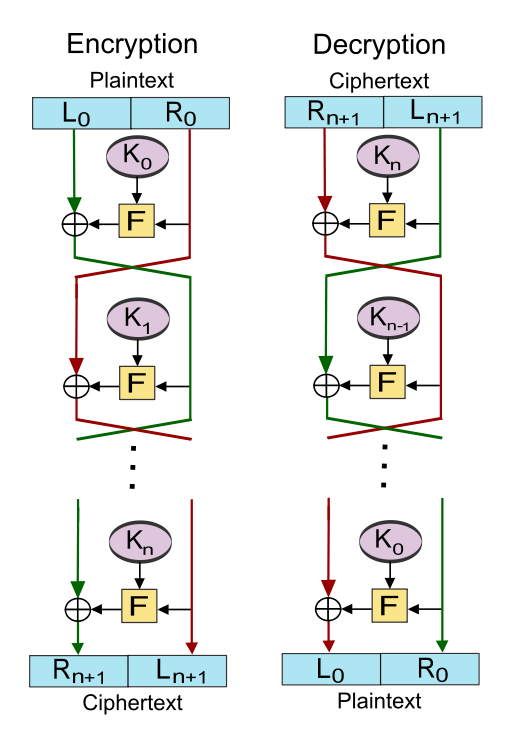
\includegraphics[scale = 0.4]{./Pictures/Feistel_cipher} % x compreso tra 0 e 1
\caption{Feistel cipher}
\label{fig:Feistel cipher}
\end{figure}

Blowfish, unlike DES, uses key-dependend S-boxes, which make it stronger.

\begin{figure}[H]
\centering
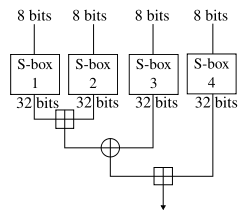
\includegraphics[scale = 0.6]{./Pictures/Blowfish_F_Function} % x compreso tra 0 e 1
\caption{F function}
\label{fig:F function}
\end{figure}

\section{Initial implementation}
Since cryptography is very a complex subject and it's very easy to introduce bugs or vulnerabilities while implementing such an algorithm, I choose to start from the single-threaded reference implementation written by Paul Kocher (https://www.schneier.com/code/bfsh-koc.zip), which has already been verified and tested, and work to make it multi-threaded.
The oroginal API is composed of three functions:

\begin{center}
\begin{lstlisting}
void Blowfish_Init(BLOWFISH_CTX *ctx, unsigned char *key, int keyLen);
void Blowfish_Encrypt(BLOWFISH_CTX *ctx, uint32_t *xl, uint32_t *xr);
void Blowfish_Decrypt(BLOWFISH_CTX *ctx, uint32_t *xl, uint32_t *xr);
\end{lstlisting}
\end{center}

The first has to be executed at the beginning, before encrypting or decrypting, it initialize the Blowfish context (like the S-boxes) using the provided key. This context structure will have to be passed to the encryption/decryption function along with the 64 bits block.\\
The block has to be passed as a pointer to the two halves associated to the two branch of the Feistel cipher, therefore the data passed to the functions is overwritten by the functions themselves. But the fact that the 64 bits block has to be split is an internal implementation detail which the user of the algorithm doesn't care and should be hidden. So I decided to implement two wrappers which take as arguments only the context and the whole 64 bits block, moreover the block is passed by value and the result is returned, in order to give the programmer the freedom to choose if overwrite the input value or not.

\begin{center}
\begin{lstlisting}
uint64_t BlowfishEncryption(BLOWFISH_CTX *ctx, uint64_t x);
uint64_t BlowfishDecryption(BLOWFISH_CTX *ctx, uint64_t x);
\end{lstlisting}
\end{center}

I also switched the entire implementation to the stdint's types which ensure better stability porting the code on different architectures and more predictable results about the underlying representation of the variables.
